\documentclass{article}
\usepackage[letterpaper, total={6in, 8in}]{geometry}
\usepackage[utf8]{inputenc}
\usepackage[hashEnumerators, smartEllipses]{markdown}
\usepackage{natbib}
\usepackage{graphicx}
\usepackage{enumitem}
\usepackage{hyperref}
\usepackage{float}
\usepackage[table,xcdraw]{xcolor}
\usepackage{bookmark}
\usepackage{listings}
\usepackage{algpseudocode}
\usepackage{algorithm}

\title{CS 2300 Database Project \\ Phase III}
\author{Jack Kufa}
\date{\today}

\begin{document}
\maketitle

\section*{Problem Statement}
I am building a Discord bot paired with a simple website, made to manage and automate a Pokemon Draft League. A Pokemon Draft League is a custom game mode
for Pokemon battling, where coaches form teams and draft unique Pokemon to compete head to head. Creating an application to automate 
the internal work involved in running such a league would be extremely helpful in streamlining specific aspects of league upkeep such as updating rankings,
tracking player wins, etc. The reason I am using a Discord bot to interface with the database
is because Discord is a vital platform for communication between players in this system, and being able to query data in the same
application as everything else related to the league would be very convenient. With that said, a simple website would be helpful for visualizing certain sets of information,
such as the League's schedule and list of Pokemon that can be drafted or have already been drafted.

\section*{Revised ER Model}S
% 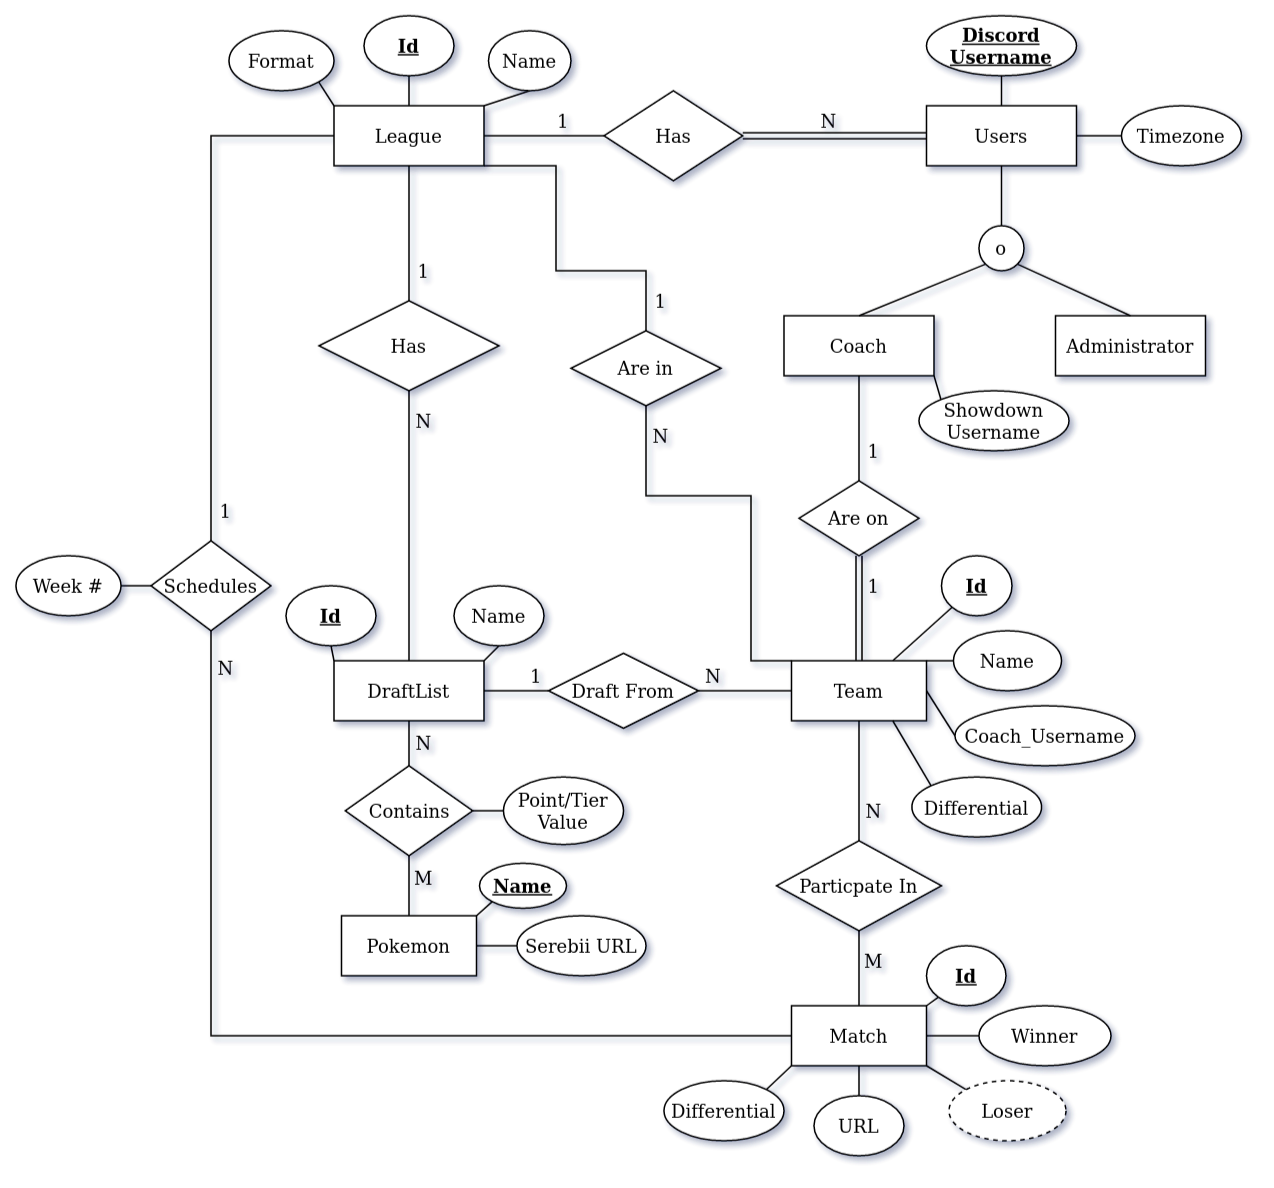
\includegraphics[scale=.38]{PokemonDraftLeagueDB_final.png}

The five entity sets are as follows:
\begin{enumerate}
    \item League: Primary entity that specifies league rules and battle format (single or double battle).
    \item Users: Users who are participating in the league. The subclasses are as follows: \begin{enumerate}
        \item Coach: Think of it like the coach of a sports team. These are the players that are participating in the league
        \item Administrator: A person who has additional privileges for managing the league.
    \end{enumerate}
    These subclasses are overlapping, meaning an Administrator can also be a coach.
    \item Teams: Consist of a coach and Pokemon, and participate in matches. This is the equivalent of a sports team.
    \item Pokemon: Entities who are listed on the draft list, sorted by tier/point value, and are chosen by teams for battling. These are like the players for a sports team.
    \item Matches: contains information related to the games being played between 2 teams.
\end{enumerate}
\section*{Logical Database Design}
% \includegraphics[scale=.38]{Logical_DB_final.png}\newpage
\section*{Summary of Data Types}
\begin{table}[H]
    \large
    \centering
    \begin{tabular}{|l|l|l|l|}
    \hline
    {\color[HTML]{2E3436} \textbf{Table}} & {\color[HTML]{2E3436} \textbf{Attribute}} & {\color[HTML]{2E3436} \textbf{Type}} & {\color[HTML]{2E3436} \textbf{Constraint}} \\ \hline
    {\color[HTML]{2E3436} League} & {\color[HTML]{2E3436} Name} & {\color[HTML]{2E3436} CHAR(50)} & {\color[HTML]{2E3436} Primary Key} \\ \hline
    {\color[HTML]{2E3436} League} & {\color[HTML]{2E3436} Format} & {\color[HTML]{2E3436} BOOLEAN} & {\color[HTML]{2E3436} } \\ \hline
    {\color[HTML]{2E3436} League\_Rules} & {\color[HTML]{2E3436} Name} & {\color[HTML]{2E3436} CHAR(20)} & {\color[HTML]{2E3436} Foreign Key} \\ \hline
    {\color[HTML]{2E3436} League\_Rules} & {\color[HTML]{2E3436} Rules} & {\color[HTML]{2E3436} CHAR(20)} & {\color[HTML]{2E3436} Multivalued} \\ \hline
    {\color[HTML]{2E3436} User} & {\color[HTML]{2E3436} Discord\_Username} & {\color[HTML]{2E3436} CHAR(32)} & {\color[HTML]{2E3436} Primary Key} \\ \hline
    {\color[HTML]{2E3436} User} & {\color[HTML]{2E3436} Timezone} & {\color[HTML]{2E3436} CHAR(5)} & {\color[HTML]{2E3436} } \\ \hline
    {\color[HTML]{2E3436} Coach} & {\color[HTML]{2E3436} Discord\_Username} & {\color[HTML]{2E3436} CHAR(32)} & {\color[HTML]{2E3436} Foreign Key} \\ \hline
    {\color[HTML]{2E3436} Coach} & {\color[HTML]{2E3436} Showdown\_Username} & {\color[HTML]{2E3436} CHAR(18)} & {\color[HTML]{2E3436} } \\ \hline
    {\color[HTML]{2E3436} Administrator} & {\color[HTML]{2E3436} Discord\_Username} & {\color[HTML]{2E3436} CHAR(32)} & {\color[HTML]{2E3436} Foreign Key} \\ \hline
    {\color[HTML]{2E3436} Team} & {\color[HTML]{2E3436} Name} & {\color[HTML]{2E3436} CHAR(50)} & {\color[HTML]{2E3436} Primary Key} \\ \hline
    {\color[HTML]{2E3436} Pokemon} & {\color[HTML]{2E3436} Name} & {\color[HTML]{2E3436} CHAR(20)} & {\color[HTML]{2E3436} Primary Key} \\ \hline
    {\color[HTML]{2E3436} Pokemon} & {\color[HTML]{2E3436} Serebii URL} & {\color[HTML]{2E3436} CHAR(120)} & {\color[HTML]{2E3436} } \\ \hline
    {\color[HTML]{2E3436} Pokemon} & {\color[HTML]{2E3436} Value} & {\color[HTML]{2E3436} INTEGER} & {\color[HTML]{2E3436} } \\ \hline
    {\color[HTML]{2E3436} Match} & {\color[HTML]{2E3436} ID} & {\color[HTML]{2E3436} CHAR(25)} & {\color[HTML]{2E3436} Primary Key} \\ \hline
    {\color[HTML]{2E3436} Match} & {\color[HTML]{2E3436} Winner} & {\color[HTML]{2E3436} CHAR(50)} & {\color[HTML]{2E3436} } \\ \hline
    {\color[HTML]{2E3436} Match} & {\color[HTML]{2E3436} Differential} & {\color[HTML]{2E3436} INTEGER} & {\color[HTML]{2E3436} } \\ \hline
    {\color[HTML]{2E3436} Schedules} & {\color[HTML]{2E3436} League\_Name} & {\color[HTML]{2E3436} CHAR(50)} & {\color[HTML]{2E3436} Foreign Key} \\ \hline
    {\color[HTML]{2E3436} Schedules} & {\color[HTML]{2E3436} Match\_ID} & {\color[HTML]{2E3436} CHAR(25)} & {\color[HTML]{2E3436} Foreign Key} \\ \hline
    {\color[HTML]{2E3436} Schedules} & {\color[HTML]{2E3436} Week\_No} & {\color[HTML]{2E3436} INTEGER} & {\color[HTML]{2E3436} } \\ \hline
    {\color[HTML]{2E3436} Team\_Pokemon} & {\color[HTML]{2E3436} Pokemon\_Name} & {\color[HTML]{2E3436} CHAR(20)} & {\color[HTML]{2E3436} Foreign Key} \\ \hline
    {\color[HTML]{2E3436} Team\_Pokemon} & {\color[HTML]{2E3436} Team\_Name} & {\color[HTML]{2E3436} CHAR(50)} & {\color[HTML]{2E3436} Foreign Key} \\ \hline
    {\color[HTML]{2E3436} Match\_Team} & {\color[HTML]{2E3436} Team\_Name} & {\color[HTML]{2E3436} CHAR(50)} & {\color[HTML]{2E3436} Foreign Key} \\ \hline
    {\color[HTML]{2E3436} Match\_Team} & {\color[HTML]{2E3436} Match\_ID} & {\color[HTML]{2E3436} CHAR(25)} & {\color[HTML]{2E3436} Foreign Key} \\ \hline
    {\color[HTML]{2E3436} Match\_Players} & {\color[HTML]{2E3436} Match\_ID} & {\color[HTML]{2E3436} CHAR(25)} & {\color[HTML]{2E3436} Foreign Key} \\ \hline
    {\color[HTML]{2E3436} Match\_Players} & {\color[HTML]{2E3436} Winner} & {\color[HTML]{2E3436} CHAR(50)} & {\color[HTML]{2E3436} From players} \\ \hline
    {\color[HTML]{2E3436} Match\_Players} & {\color[HTML]{2E3436} Loser} & {\color[HTML]{2E3436} CHAR(50)} & {\color[HTML]{2E3436} From players} \\ \hline
    {\color[HTML]{2E3436} League\_Users} & {\color[HTML]{2E3436} League\_Name} & {\color[HTML]{2E3436} CHAR(20)} & {\color[HTML]{2E3436} Foreign Key} \\ \hline
    {\color[HTML]{2E3436} League\_Users} & {\color[HTML]{2E3436} Users\_Name} & {\color[HTML]{2E3436} CHAR(32)} & {\color[HTML]{2E3436} Foreign Key} \\ \hline
    {\color[HTML]{2E3436} Coach\_Team} & {\color[HTML]{2E3436} Coach\_Username} & {\color[HTML]{2E3436} CHAR(32)} & {\color[HTML]{2E3436} Foreign Key} \\ \hline
    {\color[HTML]{2E3436} Coach\_Team} & {\color[HTML]{2E3436} Team\_Name} & {\color[HTML]{2E3436} CHAR(50)} & {\color[HTML]{2E3436} Foreign Key} \\ \hline
    \end{tabular}
\end{table}
\section*{Functionality}
The following is psuedocode for functions that will be implemented into the project. 
Please note that while the query syntax is made to mimic SQL, it is not 100\% the same syntactically, and should not be treated as such.
\begin{itemize}
    \item \textsc{Basic Functions:}
    \begin{enumerate}
        \item Draft Pokemon: 
        \begin{algorithm}[H]
            \verb|!select <Pokemon Name>|
            \label{pseudoPSO}
            \begin{algorithmic}
                \Function {Select\_Pokemon}{$discord\_username$, $user\_message$}
                \If{POKEMON \textbf{contains} $user\_message$}
                \State{$pokemon$ = \textbf{SELECT} $Name$ \textbf{FROM} POKEMON}
                \State{\quad\quad\quad\quad\quad \textbf{WHERE} $Name=user\_message$}
                \State{$coach$ = \textbf{SELECT} $Name$ \textbf{FROM} COACH}
                \State{\quad\quad\quad\quad\textbf{WHERE} $Name=discord\_username$}
                \State{\textbf{INSERT INTO} POKEMON\_COACH $Pokemon\_Name$, $Team\_Name$}
                \State{\textbf{VALUES} $pokemon$, $coach$}
                \State{\textbf{print} "You selected: " + $pokemon$}
                \Else{ \textbf{print } "ERROR. That is not a valid Pokemon!"}
                \EndIf
                \EndFunction
            \end{algorithmic}
        \end{algorithm}
        \item Submit Replay: 
        \begin{algorithm}[H]
            \verb|!submit <Replay URL>|
            \label{pseudoPSO}
            \begin{algorithmic}
                \Function {Submit\_Replay}{$user\_message$}
                \If{$user\_message$ \textbf{starts with} https://replay...}
                \State{Parse website data for $winner$, $loser$, $differential$, and $id$}
                \State{\textbf{INSERT INTO} MATCH $ID$, $Differential$}
                \State{\textbf{VALUES} $id$, $differential$}
                \State{\textbf{INSERT INTO} MATCH\_PLAYERS $Winner$, $Loser$}
                \State{\textbf{VALUES} $winner$, $loser$}
                \EndIf
                \EndFunction
            \end{algorithmic}
        \end{algorithm}
        \item Replace (Modify) drafted Pokemon:
        \begin{algorithm}[H]
            \verb|!redraft <Pokemon Name 1> <Pokemon Name 2>|
            \label{pseudoPSO}
            \begin{algorithmic}
                \Function {Redraft\_Pokemon}{$discord\_username$, $user\_message$}
                \State{\textbf{Split} $user\_message$ \textbf{into} $find$ \textbf{and} $replace$}
                \If{POKEMON \textbf{contains} $replace$}
                \State{$find\_pokemon$ = \textbf{SELECT} $Name$ \textbf{FROM} POKEMON}
                \State{\quad\quad\quad\quad\quad\quad\quad\quad \textbf{WHERE} $Name=find$}
                \State{$replace\_pokemon$ = \textbf{SELECT} $Name$ \textbf{FROM} POKEMON}
                \State{\quad\quad\quad\quad\quad\quad\quad\quad\quad\textbf{WHERE} $Name=replace$}
                \State{\textbf{UPDATE } $POKEMON\_COACH$}
                \State{\textbf{SET } $Pokemon\_Name=replace$}
                \State{\textbf{WHERE }$Pokemon\_Name=find$}
                \State{\textbf{print } $find$ + " Has been replaced with " + $replace$}
                \Else{\textbf{ print } "ERROR. That is not a valid Pokemon!"}
                \EndIf
                \EndFunction
            \end{algorithmic}
        \end{algorithm}
        \item Delete Pokemon:
        \begin{algorithm}[H]
            \verb|!delete <Pokemon Name>|
            \label{pseudoPSO}
            \begin{algorithmic}
                \Function {Delete\_Pokemon}{$discord\_username$, $user\_message$}
                \If{USER\_ADMINISTRATOR$.contains(discord\_username)$}
                \State{\textbf{DELETE FROM} POKEMON \textbf{WHERE} Pokemon$.Name=user\_message$}
                \EndIf
                \EndFunction
            \end{algorithmic}
        \end{algorithm}
    \end{enumerate}
    \item \textsc{General Queries:}
    \begin{enumerate}
        \item Query all of a user's usernames:
        \begin{algorithm}[H]
            \verb|!userinfo <User>|
            \label{pseudoPSO}
            \begin{algorithmic}
                \Function {User\_Info}{$user\_message$}
                \If{USER \textbf{contains} $user\_message$}
                \State{R$1$ = \textbf{INNER JOIN} USER$.Discord\_Username$ = COACH$.Discord\_Username$}
                \State{$R2$ = \textbf{INNER JOIN} R1$.Discord\_Username$ = COACH\_TEAM$.Coach\_Username$}
                \State{$info$ = \textbf{SELECT} $Discord\_Username, Team\_Name, Showdown\_Name$ \textbf{FROM} $R2$}
                \State{\qquad\quad \textbf{ WHERE }$Discord\_Name=user\_message$}
                \State {\textbf{print } $info$}
                \EndIf
                \EndFunction
            \end{algorithmic}
        \end{algorithm}
        \item Query differential:
        \begin{algorithm}[H]
            \verb|internal function|
            \label{pseudoPSO}
            \begin{algorithmic}
                \Function {Differential}{$team\_name$}
                \State{$positive$ = \textbf{SELECT SUM} $Differential$ \textbf{FROM} MATCH}
                \State{\qquad\qquad\quad \textbf{WHERE} MATCH.$Winner=team\_name$}
                \State{$negative$ = \textbf{SELECT SUM} $Differential$ \textbf{FROM} MATCH}
                \State{\qquad\qquad\quad \textbf{WHERE} MATCH.$Loser=team\_name$}
                \State{\textbf{return} $positve-negative$}
                \EndFunction
            \end{algorithmic}
        \end{algorithm}
        \item Query wins:
        \begin{algorithm}[H]
            \verb|internal function|
            \label{pseudoPSO}
            \begin{algorithmic}
                \Function {Wins}{$team\_name$}
                \State{$teamIDs$ = \textbf{SELECT} $Match\_ID$ \textbf{FROM} MATCH\_TEAM}
                \State{\qquad\qquad \textbf{ WHERE} $Team\_Name=team\_name$}
                \State{$wins$ = \textbf{SELECT COUNT} $Winner$ \textbf{FROM} MATCH\_PLAYERS}
                \State{\qquad\quad \textbf{ WHERE} $ID=teamIDs$}
                \State{\textbf{return} $wins$}
                \EndFunction
            \end{algorithmic}
        \end{algorithm}
        \item Query rankings:
        \begin{algorithm}[H]
            \verb|!rankings|
            \label{pseudoPSO}
            \begin{algorithmic}
                \Function {Rankings}{}
                \State{$rankings$ = \textbf{SELECT} $team$ \textbf{FROM} TEAM}
                \State{\qquad\qquad\quad \textbf{ORDERBY} $\textsc{Differential($team$)}+\textsc{Wins($teams$)}$}
                \State{\qquad\qquad\qquad\qquad\qquad\quad  $ > \textsc{Differential($previous\_team$)}+\textsc{Wins($previous\_teams$)}$}
                \State{print $rankings$}
                \EndFunction
            \end{algorithmic}
        \end{algorithm}
        \item Query matches played:
        \begin{algorithm}[H]
            \verb|!matchesplayed|
            \label{pseudoPSO}
            \begin{algorithmic}
                \Function {Matches\_Played}{}
                \State{$matches$ = \textbf{SELECT} $ID$ \textbf{FROM} MATCH}
                \State{\qquad \textbf{ WHERE $ID != NULL$} }
                \State{\textbf{print} $matches$ as URL}
                \EndFunction
            \end{algorithmic}
        \end{algorithm}
        \item Query specific Pokemon:
        \begin{algorithm}[H]
            \verb|!pokemon <Pokemon Name>|
            \label{pseudoPSO}
            \begin{algorithmic}
                \Function {Query\_Pokemon}{$user\_message$}
                \If{POKEMON \textbf{contains} $user\_message$}
                \State{$pokemon$ = \textbf{SELECT} $Name$ \textbf{FROM} POKEMON}
                \State{\quad\quad\quad\quad\quad \textbf{WHERE} $Name=user\_message$}
                \State{\textbf{print} $pokemon$}
                \Else{ \textbf{print } "ERROR. That is not a valid Pokemon!"}
                \EndIf
                \EndFunction
            \end{algorithmic}
        \end{algorithm}
        \item Query Average Differential:
        \begin{algorithm}[H]
            \verb|!average |
            \label{pseudoPSO}
            \begin{algorithmic}
                \Function {Average}{}
                \State{\textbf{SELECT AVG} $Differential$ \textbf{FROM} MATCH}
                \EndFunction
            \end{algorithmic}
        \end{algorithm}
    \end{enumerate}
\end{itemize}
    This Functionality is tentative, and will change as the project evolves over time.
\end{document}
    